% This file is modified by Frans Oliehoek <faolieho@science.uva.nl>
% on 2005/12/18. (original file name: conference-ornate-20min.en.tex)

\documentclass[11pt]{beamer}

% This file is a solution template for:

% - Talk at a conference/colloquium.
% - Talk length is about 20min.
% - Style is ornate.



% Copyright 2004 by Till Tantau <tantau@users.sourceforge.net>.
%
% In principle, this file can be redistributed and/or modified under
% the terms of the GNU Public License, version 2.
%
% However, this file is supposed to be a template to be modified
% for your own needs. For this reason, if you use this file as a
% template and not specifically distribute it as part of a another
% package/program, I grant the extra permission to freely copy and
% modify this file as you see fit and even to delete this copyright
% notice. 


\mode<presentation>
{
\usetheme{CambridgeUS}
%\usetheme{IAS_sidebar} 	% only a simple left side bar, frame-title box varies in size when using subtitles for frames.
%\usetheme{IAS_sidebar2_10pt} 	% only a simple side bar, the frame-title box has a fixed size to exactly fit a title and subtitle. For usage with 10pt font, i.e.: \documentclass[10pt]{beamer}
%\usetheme{IAS_sidebar2_11pt} 	% As above only changed to fit 11pt fonts.
%\usetheme{IAS_sidebar2_12pt} 	% As above only changed to fit 12pt fonts.
%\usetheme{IAS_sidebarNav} 	% An IAS side bar with navigation
%\usetheme{IAS_topNav}		% Only top navigation with IAS colors
%\usetheme{IAS_topNav_bottomAuthorTitle}	%Top navigation and author/title in the bottom with IAS colors
%\usetheme{IAS_topNav_leftIASbar_10pt}	% both top navigation and the IAS sidebar, the frame-title box has a fixed size to exactly fit a title and subtitle. For usage with 10pt font, i.e.: \documentclass[10pt,english
%\usetheme{IAS_topNav_leftIASbar_11pt}	% As above only changed to fit 11pt fonts.
%\usetheme{IAS_topNav_leftIASbar_12pt}	% As above only changed to fit 12pt fonts.
  \setbeamercovered{transparent}
%   % or whatever (possibly just delete it)
}


% to remove the navigation symbols:
%\setbeamertemplate{navigation symbols}{}

\usepackage[T1]{fontenc} % Ligaturen, richtige Umlaute im PDF
\usepackage[utf8]{inputenc}% UTF8-Kodierung für Umlaute usw

\usepackage[ngerman, american]{babel}
% or whatever

\usepackage{times}
\usepackage[T1]{fontenc}
% Or whatever. Note that the encoding and the font should match. If T1
% does not look nice, try deleting the line with the fontenc.

\usepackage{amsmath,amssymb,amstext,mathtools,siunitx}


\title [Coop. eff. in motor-driven cargo transport] %(optional, use only with long paper titles)
{Cooperative effects\\ in motor-driven cargo transport}

%\subtitle
%{Ein kleiner Einblick}

\author % (optional, use only with lots of authors)
{Kevin Klein}
%{F.~Author\inst{1} \and S.~Another\inst{2}}
% - Give the names in the same order as the appear in the paper.
% - Use the \inst{?} command only if the authors have different
%   affiliation.

\institute[Universität des Saarlandes] % (optional, but mostly needed)
{
Naturwissenschaftlich-Technische Fakultät II \\
- Physik und Mechatronik -  \\
Universität des Saarlandes \\
%  \inst{1}%
%  Department of Computer Science\\
%  University of Somewhere
%  \and
%  \inst{2}%
%  Department of Theoretical Philosophy\\
%  University of Elsewhere}
% - Use the \inst command only if there are several affiliations.
% - Keep it simple, no one is interested in your street address.
}

\date[01.12.2016] % (optional, should be abbreviation of conference name)
{Vortrag zur Bachelorarbeit, 2016}
% - Either use conference name or its abbreviation.
% - Not really informative to the audience, more for people (including
%   yourself) who are reading the slides online

\subject{Bachelorarbeit Physik}
% This is only inserted into the PDF information catalog. Can be left
% out. 


% If you have a file called "university-logo-filename.xxx", where xxx
% is a graphic format that can be processed by latex or pdflatex,
% resp., then you can add a logo as follows:

 %\pgfdeclareimage[height=0.5cm]{UdS-Logo}{Logo-uni-Saarland_03}
 %\logo{\pgfuseimage{UdS-Logo}}
%\pgfdeclareimage[height=0.5cm]{institution-logo}{uva_logo}
%\logo{\pgfuseimage{institution-logo}}



% Delete this, if you do not want the table of contents to pop up at
% the beginning of each subsection:
\AtBeginSubsection[]
{
  \begin{frame}<beamer>
    \frametitle{Overview}
    \tableofcontents[currentsection,currentsubsection]
  \end{frame}
}


% If you wish to uncover everything in a step-wise fashion, uncomment
% the following command: 

%\beamerdefaultoverlayspecification{<+->}


\begin{document}

\begin{frame}
  \titlepage
\end{frame}

\begin{frame}
  \frametitle{Overview}
  \tableofcontents
  % You might wish to add the option [pausesections]
\end{frame}


% Structuring a talk is a difficult task and the following structure
% may not be suitable. Here are some rules that apply for this
% solution: 

% - Exactly two or three sections (other than the summary).
% - At *most* three subsections per section.
% - Talk about 30s to 2min per frame. So there should be between about
%   15 and 30 frames, all told.

% - A conference audience is likely to know very little of what you
%   are going to talk about. So *simplify*!
% - In a 20min talk, getting the main ideas across is hard
%   enough. Leave out details, even if it means being less precise than
%   you think necessary.
% - If you omit(weglassen) details that are vital to the proof/implementation,
%   just say so once. Everybody will be happy with that.

%\section{Motivation}
\section{Introduction}

%\subsection{The Basic Problem That We Studied}
\subsection{Motivation}

\begin{frame}
  %\frametitle{Make Titles Informative.}
  %\framesubtitle{Subtitles are optional.}
  % - A title should summarize the slide in an understandable fashion
  %   for anyone how does not follow everything on the slide itself.
  \frametitle{Intracellular Cargo Transport}
  %\framesubtitle{Subtitles are optional.}

%  \begin{itemize}
%  \item
%   Use \texttt{itemize} a lot.
%  \item
%    Use very short sentences or short phrases.
%  \end{itemize}
  \begin{itemize}
  \item
    Cells need to be able to rearrange or move cargos in its interior (e.g. nutrients, organelles)
    \pause
  \item
    Motorproteins (here: kinesin and dynein) pull the cargo along filaments (here: microtubules)
  \end{itemize}
  \begin{center}
    \includegraphics<2->[scale=0.3]{img/cargo-transport.png}
  \end{center}
\end{frame}
  
\begin{frame}
\frametitle{Intracellular Cargo Transport}
  \begin{itemize}
  \item
   Bi- and unidirectional transport subject of much research
   \pause
  \item
   Different attempts of modeling these kinds of transport
   \pause
  \item
   Here: closer look at so called mean-field model and explicit-motor-positions model
  \end{itemize}
\end{frame}


\subsection{The mean-field model by Li et al.}

% \begin{frame}
%   \frametitle{The model}
% %   You can create overlays\dots
% %   \begin{itemize}
% %   \item using the \texttt{pause} command:
% %     \begin{itemize}
% %     \item
% %       First item.
% %       \pause
% %     \item    
% %       Second item.
% %     \end{itemize}
% %   \item
% %     using overlay specifications:
% %     \begin{itemize}
% %     \item<3->
% %       First item.
% %     \item<4->
% %       Second item.
% %     \end{itemize}
% %   \item
% %     using the general \texttt{uncover} command:
% %     \begin{itemize}
% %       \uncover<5->{\item
% %         First item.}
% %       \uncover<6->{\item
% %         Second item.}
% %     \end{itemize}
% %   \end{itemize}
%   \begin{itemize}
%   \item
%    Two teams: slow and fast kinesin motors\\
%    \begin{center}
%       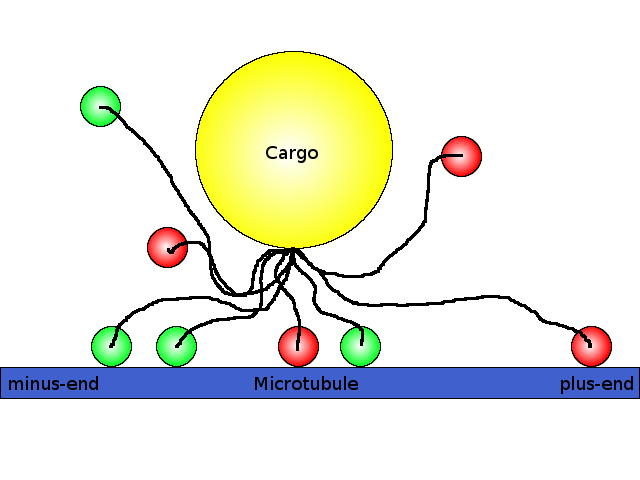
\includegraphics[scale=0.3]{img/cargo-transport.png}
%    \end{center}
%   \item
%    Different motor parameters
%   \end{itemize}
% \end{frame}

\begin{frame}
  \frametitle{The model}
  \begin{itemize}
  \item
    One slow and one fast team of kinesins pulling the cargo \pause
  \item
    $N_f$ and $N_s$ motors available, $n_f$ and $n_s$ numbers of bound motors \pause
  \item
    Force independent binding rates $\pi_{0s}$ and $\pi_{0f}$
    \pause
  \item
    Force dependent unbinding rates\\
    \begin{equation*}
     \epsilon\left(F\right) = \epsilon_{0} exp\left({\frac{F}{F_{d}}}\right)
    \end{equation*}
    \pause
  \item
    Force dependent velocities
    \begin{equation*}\label{e.linear-velocity}
    \begin{aligned}
      V_s\left(F\right) &= v_s \left(1 - F/F_{ss}\right) \qquad \phantom{_{ff}} \text{for} \quad F \leq 0 < F_{ss} \\
      V_f\left(F\right) &= v_f \left(1 - F/F_{sf}\right) \qquad \phantom{_{ss}} \text{for} \quad 0 \leq F < F_{sf},
    \end{aligned}
    \end{equation*}
  \end{itemize}  
\end{frame}

\begin{frame}
 \frametitle{The model}
 \begin{itemize}
  \item
    Assumption of force balance and equal force sharing\\
    \begin{equation*}\label{e.force-balance}
      n_fF_+ = -n_sF_- \equiv F\left(n_f, n_s\right),
    \end{equation*}
    \pause
  \item
    Assumption of equal velocities of all motors\\
    \begin{equation*}\label{e.equal-velocities}
      V_s\left(F_-\right) = V_f\left(F_+\right) = v\left(n_f, n_s\right),
    \end{equation*}
    \pause  
  \item
    These lead to the transport velocity\\
    \begin{equation*}\label{e.mt-velocity}
      v\left(n_f, n_s\right) = \frac{v_sv_f}{\left(1 - \dfrac{n_f}{n}\right)v_f + \dfrac{n_f}{n}v_s},
    \end{equation*}
    uniquely determined by the numbers $n_f$ and $n_s$
 \end{itemize}
\end{frame}


\begin{frame}
  \frametitle{Results}
  \begin{itemize}
  \item
    By using different sets of motor parameters Li \textit{et al.} find three distinct motility regimes\\
    \begin{center}
      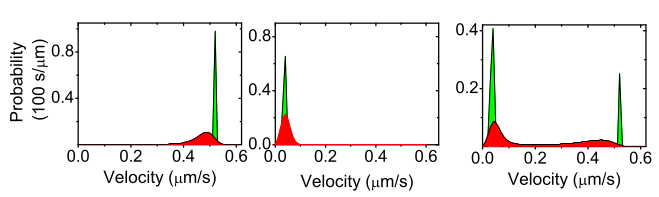
\includegraphics[scale=0.55]{img/li-velocity-distribution.png}
    \end{center}
    \pause
  \item
    Bimodal state explained by small detachment to stall force ratio $\frac{F_d}{F_s}$ and resulting unbinding cascades
  \end{itemize}
%   \begin{columns}
%   \column[c]{.45\textwidth}
%     \uncover<3->{\begin{block}{Quantenmech. Oszillator}
%       \begin{equation}
%         E_{vib}(n) = \hbar \omega \left(n + \frac{1}{2}\right)
%       \end{equation}	  
%     \end{block}
%     }    
%     \column[c]{.45\textwidth}
%     \uncover<3->{\begin{block}{Quantenmech. Rotator}
%       \begin{equation}
%         E_{rot}(J) = \frac{\hbar^2}{2I} J\left(J+1\right)
%       \end{equation}	  
%     \end{block}
%     }
%    \end{columns}
%   \uncover<4->{
%     ¸\begin{block}{Gesamtenergie}
%        \begin{equation}
%          E = \hbar \omega \left(n + \frac{1}{2}\right) + \frac{\hbar^2}{2I} J\left(J+1\right)
%        \end{equation}
%      \end{block}
%   }
\end{frame}

\subsection{Discussion}

\begin{frame}
  \frametitle{Problems}
 \begin{itemize}
  \item 
    Equal force sharing and equal motor velocities?
    \pause
  \item
    => all motors within one team need to be at the exact same position
    \pause
  \item
    => the system of motors and cargo is always stepping as a complete unit
    \pause
  \item
    -> unrealistic scenario
 \end{itemize}
\end{frame}

\begin{frame}
  \frametitle{Idea}
  \begin{itemize}
   \item 
     Introducing a new model which takes the explicit motor positions into account
   \item
     Comparing the results of this explicit model to the results of the mean-field model
  \end{itemize}
\end{frame}


\section{The explicit model}

\subsection{Adjustments and comparison to the mean-field model}
\begin{frame}
  \frametitle{Adjustments}
  \begin{itemize}
   \item
     Stalks of the motors modeled as cable-like Hookean springs: slack up to a length of $L_0$ and linear force relation beyond $L_0$.\\ The force of the i-th motor on the cargo reads
     \begin{equation*}\label{e.motor-spring-relation}
	F_i =
	\begin{cases}
	  \alpha \left(x_i\left(t\right) - x_{C}\left(t\right) + L_0\right), \qquad & \qquad \phantom{\vert}x_i\left(t\right) - x_{C}\left(t\right) \phantom{\vert} < -L_0, \\
	  0,	& \qquad \vert x_i\left(t\right) - x_{C}\left(t\right) \vert < \phantom{-}L_0, \\
	  \alpha \left(x_i\left(t\right) - x_{C}\left(t\right) - L_0\right), \qquad & \qquad \phantom{\vert}x_i\left(t\right) - x_{C}\left(t\right) \phantom{\vert} > \phantom{-}L_0.
	\end{cases}
      \end{equation*}
     \pause
   \item
     Stepping rates for each motor
     \begin{equation*}\label{e.motor-stepping-rate}
      s_s\left(F_i\right) =
      \begin{dcases}
	\dfrac{v_s}{d}, \qquad & \qquad F_i < 0, \\
	\dfrac{v_s}{d}\left[1 - \frac{F_i}{F_{ss}}\right], \qquad & \qquad 0 \leq F_i \leq F_{ss}, \\
	\dfrac{v_s^B}{d}, \qquad & \qquad F_i > F_{ss}
      \end{dcases}
     \end{equation*}
  \end{itemize}

\end{frame}

\begin{frame}
 \frametitle{Comparison to results of Li \textit{et al.}}
 \begin{center}
  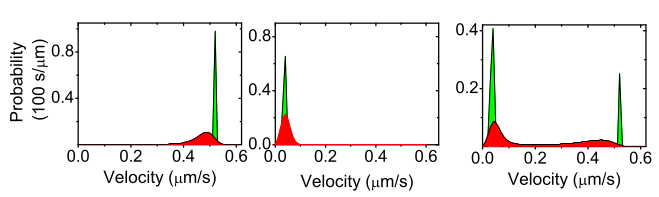
\includegraphics[scale=0.55]{img/li-velocity-distribution.png}
 \end{center}
 \begin{center}
  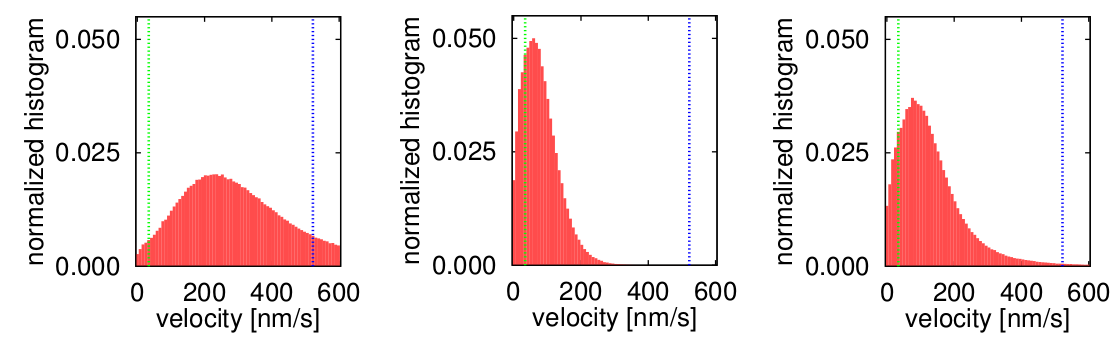
\includegraphics[scale=0.35]{img/comp-li.png}
 \end{center} 
 \begin{itemize}
  \item
    Different results for same sets of parameters!
 \end{itemize}
\end{frame}

\begin{frame}
 \frametitle{Bimodal velocity distributions?}
 \begin{itemize}
  \item 
    Are bimodal velocity distributions possible in the explicit model?
    \pause
  \item
    Yes they are, but with different sets of parameters!
    \begin{center}
      \includegraphics<2->[scale=0.55]{img/bimodal-vel-dis.png}
    \end{center}
 \end{itemize}

\end{frame}


\subsection{Analysis of the transport process}
\begin{frame}
 \frametitle{A closer look at the motor parameters}
 \begin{itemize}
  \item
    In order to understand the underlying effects, which lead to the shown bimodal velocity distribution, changes to the following parameters have been examined:
    \pause
    \begin{itemize}
     \item Slow and fast velocities $v_s$ and $v_f$ \pause
     \item Attachment rate $\kappa_a$ \pause
     \item Stall forces $F_{ss}$ and $F_{sf}$ \pause
     \item Force free detachment rate $\kappa_a^0$ \pause
     \item Detachment forces $F_{ds}$ and $F_{df}$
    \end{itemize}

 \end{itemize} 
\end{frame}

\begin{frame}
 \frametitle{Velocities, attachment rate and stall forces}
 \begin{itemize}
  \item
    Bimodal velocities: \mbox{$v_s =$ \SI[per-mode=fraction]{100}{\nano\metre\per\second}}, \mbox{$v_f =$ \SI[per-mode=fraction]{2000}{\nano\metre\per\second}}\\
    Increasing the velocity of slow motors leads to a vanishing distinctness of the bimodal velocity distribution
    \pause
  \item
    Bimodal attachment rate: \mbox{$\kappa_a =$ \SI{5}{\per\second}}\\
    For very low attachment rates (< \SI{0.1}{\per\second}) transport is stalling most of the time and is carried out by only one attached motor at a time.\\
    Very high attachment rates (> \SI{100}{\per\second}) lead to unimodal velocity distributions, as all motors are involved into transport.
    \pause
  \item
    Bimodal stall forces: \mbox{$F_{s} =$ \SI{5}{\pico\newton}}\\
    Changes to the stall force of slow motors do not effect the velocity distribution.\\
    The bimodal velocity distribution is kept for stall forces of fast motors that are larger than the detachment forces.
 \end{itemize}

\end{frame}

\begin{frame}
 \frametitle{Force free detachment rate}
 \begin{itemize}
  \item 
    Bimodal force free detachment rate: \mbox{$\kappa_d^0 = $ \SI{1}{\per\second}}
  \item
    Reminder: $\kappa_d\left(F_i\right) = \kappa_d^0 exp\left(\frac{\vert F_i\vert}{F_d}\right)$
 \end{itemize}
 
  \begin{columns}
  \column[c]{.5\textwidth}
    \begin{itemize}
     \item Bimodal for roughly \mbox{\SI{0.1}{\per\second} $\leq \kappa_d^0 \leq $ \SI{5}{\per\second}}
    \end{itemize}
  \column[c]{.5\textwidth}
    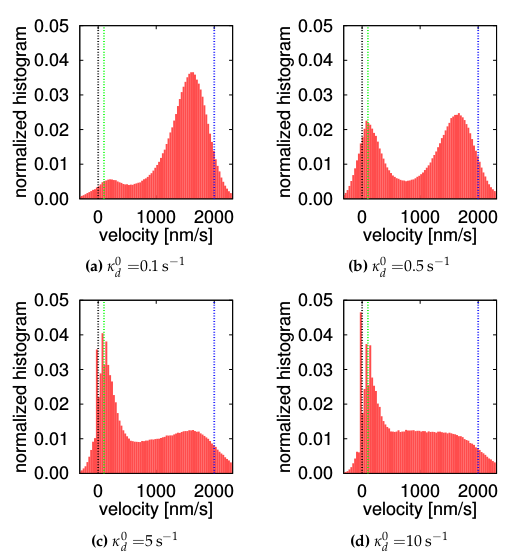
\includegraphics[scale=.37]{img/kd0.png}
 \end{columns} 
\end{frame}

\begin{frame}
 \frametitle{Detachment forces}
 \begin{itemize}
  \item 
    Bimodal detachment forces: \mbox{$F_{d} = $ \SI{1}{\pico\newton}}
  \item
    Reminder: $\kappa_d\left(F_i\right) = \kappa_d^0 exp\left(\frac{\vert F_i\vert}{F_d}\right)$
 \end{itemize}
 \begin{center}
  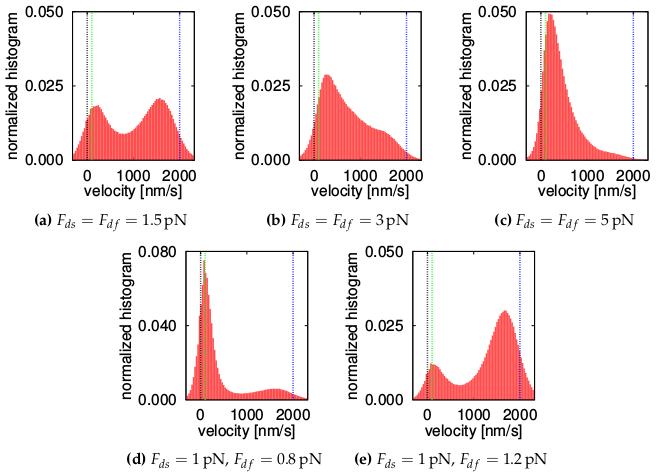
\includegraphics[scale=.4]{img/Fd.png}
 \end{center}

\end{frame}

\begin{frame}
 \frametitle{Summary of the parameter analysis}
 In order to obtain bimodal velocity distribution one needs:
 \begin{itemize}
  \item $F_{sf} > F_d$ \pause
  \item Only few motors must participate in cargo transport simultaneously \pause
  \item Detachment forces of fast and slow motors need to be ``close'' \pause
  \item A considerable gap between slow and fast motor's velocities
 \end{itemize}

\end{frame}

\begin{frame}
 \frametitle{Extension on bidirectional case}
 \begin{itemize}
  \item Bi- and even trimodal velocity distributions obtainable for symmetric motors.
 \end{itemize}

 \begin{center}
  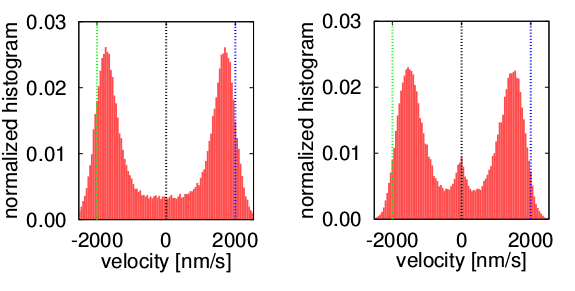
\includegraphics[scale=.6]{img/bidirectional.png}
 \end{center} 
 
\end{frame}








% \subsection{Previous Work}
% 
% \begin{frame}
%   \frametitle{Make Titles Informative.}
%   \begin{itemize}
%   \item
%     Really...
%   \end{itemize}
% \end{frame}


%\section{Our Results/Contribution}






\section{Summary}

\begin{frame}
  \frametitle<presentation>{Summary}

  % Keep the summary *very short*.
  \begin{itemize}
  \item
    Bimodal motility states have been obtained by Li \textit{et al.} using the mean field model.
  \item
    These bimodal states cannot be reproduced by an explicit model for the same set of parameters but for different sets of parameters.
  \item
    The explicit model can be extended on the bidirectional case and, there, leads to bimodal and even trimodal motility states.
  \end{itemize}

  % The following outlook is optional.
  \vskip0pt plus.5fill
  \begin{itemize}
  \item
    Further improvements:
    \begin{itemize}
    \item
      A different modeling approach for the detachment rate could be examined, as the exponential modeling heavily effects the motility state.
    \end{itemize}
  \end{itemize}
\end{frame}

\section*{}
\begin{frame}
 \begin{center}
  \begin{Huge}
   Thank you for your attention!
  \end{Huge}
 \end{center}

\end{frame}


% All of the following is optional and typically not needed. 
\appendix
\section<presentation>*{\appendixname}
\subsection<presentation>*{References}

\begin{frame}[allowframebreaks]
  \frametitle<presentation>{References}
    
  \begin{thebibliography}{10}
    
  \beamertemplatebookbibitems
  % Start with overview books.

%   \bibitem{gremlich}
%     H.~Günzler, H.-U.~Gremlich.
%     \newblock {\em IR-Spektroskopie - Eine Einführung}.
%     \newblock Wiley-VCH, 2003.
 
    
  \beamertemplatearticlebibitems
  % Followed by interesting articles. Keep the list short. 

  \bibitem{arnold}
    X. Li, R. Lipowsky, and J. Kierfeld.
    \newblock Bifurcation of Velocity Distributions in Cooperative Transport of Filaments by Fast and Slow Motors.
    \newblock {\em Biophysical Journal}, vol. 104, pp. 666–676, 2013.
  \end{thebibliography}
\end{frame}

\subsection<presentation>*{Additional material}

\begin{frame}
 \frametitle{Li \textit{et al.} parameters}
   \begin{columns}
      \column[c]{.5\textwidth}
	\begin{footnotesize}Parameters used by Li \textit{et al.} for the three different motility regimes\end{footnotesize}
	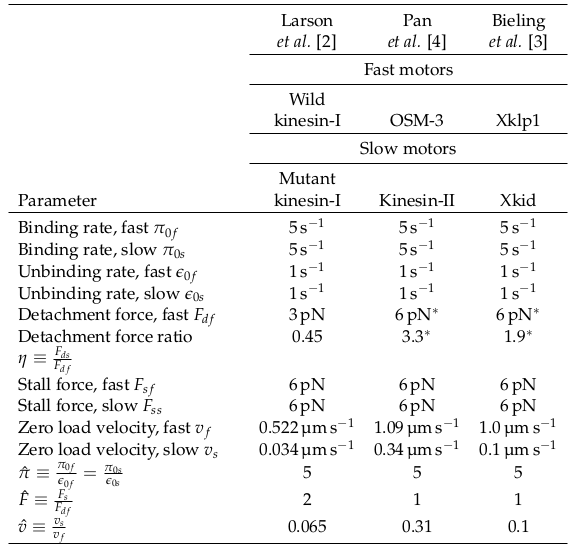
\includegraphics[scale=.4]{img/params-exp.png}
      \column[c]{.5\textwidth}
	\begin{footnotesize}Parameters used for the explicit model simulation for the bistable motility regime\end{footnotesize}
	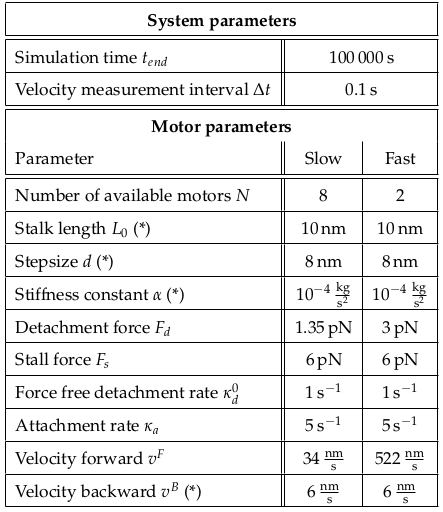
\includegraphics[scale=.4]{img/params-sim.png}
    \end{columns} 
\end{frame}

\begin{frame}
 \frametitle{Changes to parameters to obtain bimodal velocity distribution}
 \centering
 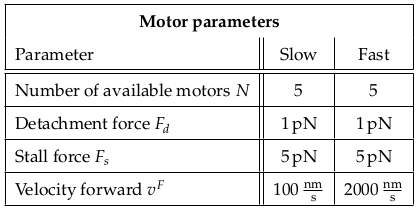
\includegraphics[scale=.5]{img/params-bimodal-changes.png} 
\end{frame}

\begin{frame}
 \frametitle{Different transport characteristics to the shown bimodal case}
 \centering
 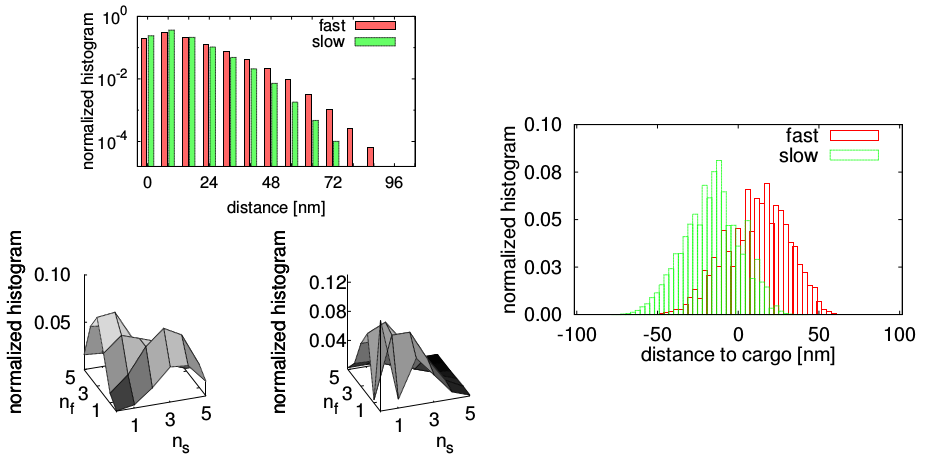
\includegraphics[scale=.5]{img/transport-characteristics.png} 
\end{frame}

\begin{frame}
 \frametitle{Simulations for differing slow motor velocities}
 \centering
 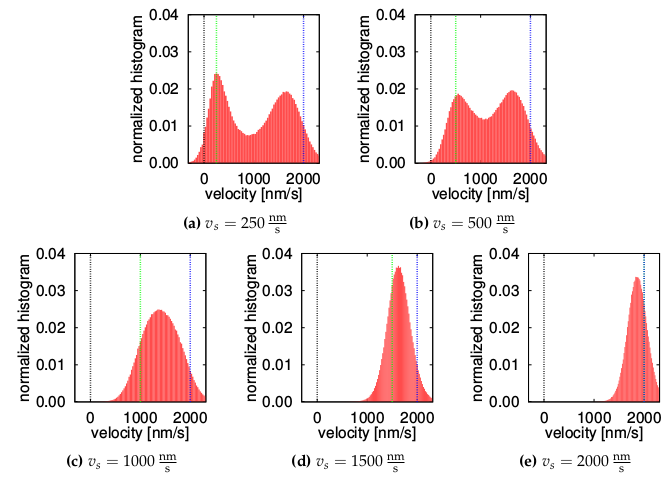
\includegraphics[scale=.5]{img/sim-velo.png} 
\end{frame}

\begin{frame}
 \frametitle{Simulations for differing attachment rates}
 \centering
 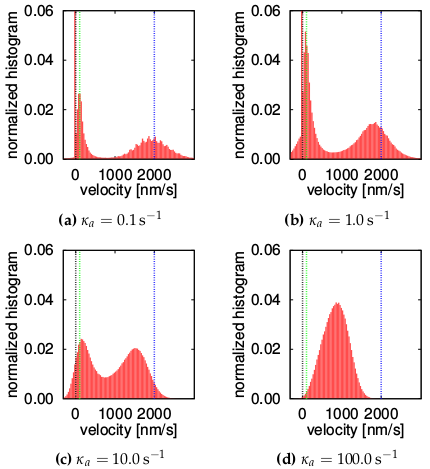
\includegraphics[scale=.5]{img/sim-ar.png} 
\end{frame}

\begin{frame}
 \frametitle{Simulations for differing stall forces of fast motors}
 \centering
 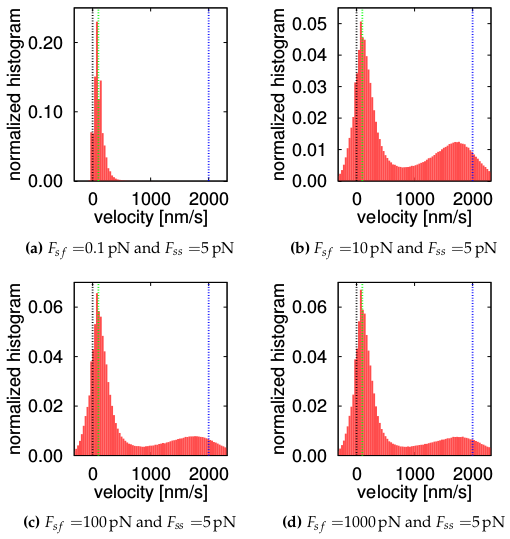
\includegraphics[scale=.5]{img/sim-sff.png} 
\end{frame}

\begin{frame}
 \frametitle{Motor distributions in the bidirectional case}
 \centering
 \begin{footnotesize}
  Bidirectional bimodal velocitiy distribution: motors attached, motors with $|F| > 0$
 \end{footnotesize}
  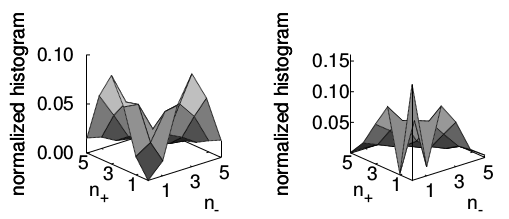
\includegraphics[scale=.5]{img/bidi-bimodal-mdist.png} \\
 \begin{footnotesize}
  Bidirectional trimodal velocitiy distribution: motors attached, motors with $|F| > 0$
 \end{footnotesize}
  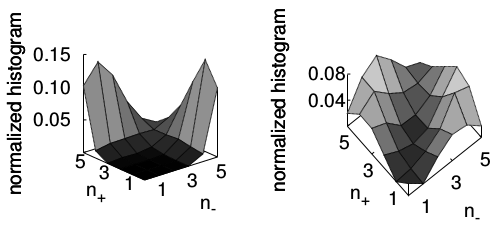
\includegraphics[scale=.5]{img/bidi-trimodal-mdist.png} 
\end{frame}

\end{document}



